\section*{Problem 4}
	\begin{proof} [Solution]
		Here are results.
		\begin{center}
			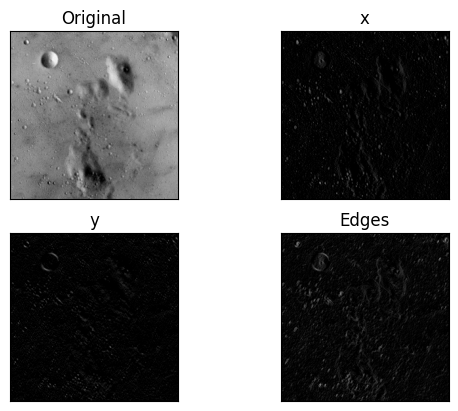
\includegraphics[width=0.65\textwidth]{moon.png}
			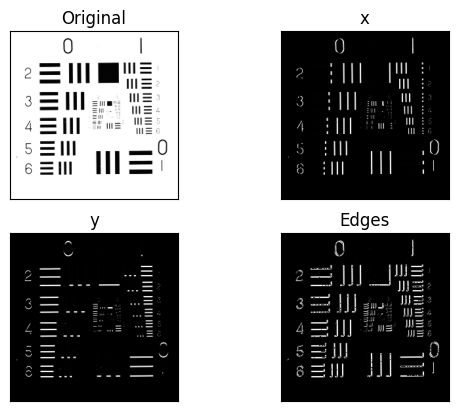
\includegraphics[width=0.65\textwidth]{resolution_table.png}
			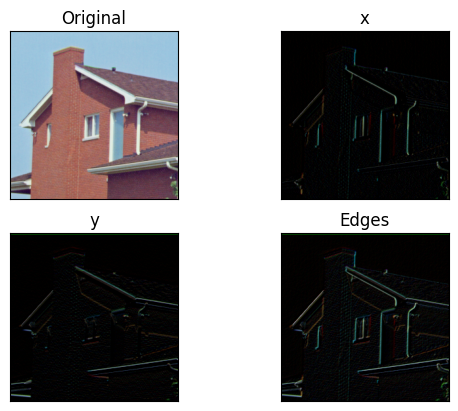
\includegraphics[width=0.65\textwidth]{house.png}
			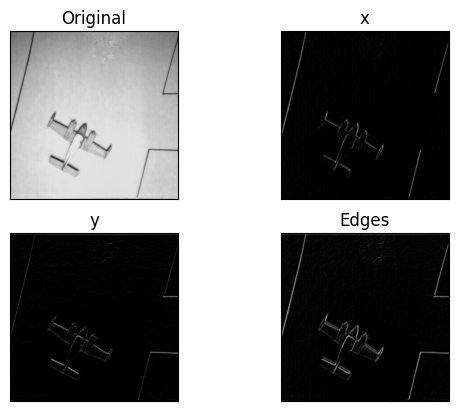
\includegraphics[width=0.65\textwidth]{airplane.png}
		\end{center}
		An idea to consider when trying to find the edge of an image is to claim that the edge is where the color intensity changes. This is quite reasonable, based on our perception. The most intuitive way to find areas where color intensity changes is to use differentiation. When calculating the first derivative along the x and y axes, the part where the derivative changes rapidly can be considered an edge.\\
		We cannot define continuous differentiation in images due to computational limitations. Therefore, we must define and use discrete differentiation. There are several finite difference methods, but I think the central difference method may be more effective because images require determining the boundary with the surroundings. Additionally, it may be difficult to process ambiguous boundaries due to noise or staircase effects. In this case, we can consider intentionally blurring the image so that the edges cannot be considered, or readjusting the image through a filter.\\
	\end{proof}